\chapter{Conceitos Iniciais}

\section{Kit de Desenvolvimento de Software (SDK)}
Kit de Desenvolvimento de Software, comumente abreviada para SDK (do inglês, Software
Development Kit) é um pacote que contém ferramentas, bibliotecas, códigos fonte,
e outros utilitarios pré criados. \cite{Thorn2008}
A Google e Apple oferecem respectivamente o Android SDK e o iOS SDK, 
que possibilitam o desenvolvimento de aplicativos para suas plataformas.


\section{Interface Gr\'afica (UI)}
Interface gráfica, comumente abreviada para UI (do inglês, User Interface) é a 
parte da aplicação que o usuário vê e com a qual ele interage. \cite{Chong2004}
A interface inclui as telas, janelas, controles, menus e etc. \cite{Chong2004}

De acordo com um estudo publicado pelo IEEE \cite{Khalid2015} sobre os motivos pelos 
quais os usuários mais reclamam de aplicações móveis, a interface gráfica é um dos 
casos mais frequentes, o que demonstra a necessidade de empenho no desenvolvimento
de interfaces agradáveis e intuitivas.

Não é de se estranhar que as empresas desenvolvedoras dos sistemas operacionais
cujas plataformas móveis são as mais competitivas no mercado ofereçam maneiras de
padronizar as interfaces dos aplicativos feitos para suas plataformas.

De fato, a Google e a Apple oferecem dentro de seus SDKs ferramentas de padronização
de interfaces. No caso da Google, esse conjunto de ferramentas
é chamado de Material Design \cite{materialdesign} e, além de ser oferecido para o Android, também
pode ser utilizada nas plataformas Web, Flutter e, inclusive, iOS.
Já a Apple, oferece seu kit gráfico, o UIKit \cite{documentationapple}, apenas para sua própria plataforma.

\section{Experiência do Usu\'ario (UX)}
Um segundo conceito muito importante quando se trata de aplicações móveis
 é a Experiência do Usuário, comumente abreviada para UX (do inglês, User 
 Experience). Apesar de ser um conceito amplamente disseminado e aceito,
 ele ainda não é bem definido ou entendido. \cite{Law2008}
 
 Entretanto, para uma certa compreensão, pode-se utilizar a definição de Hassenzahl & 
 Tractinsky:
 
 \begin{quote}
 \enquote{Experiência de usuário é a consequêcia do estado interno de um usuário
(predisposição, expectativa, necessidade, motivação, humor, etc), das
caracteristicas do sistema designado (complexibilidade, propósito, usabilidade,
funcionalidade, etc) e do contexto (ou ambiente) no qual a interação ocorre
(configuração organizacional/social, significância da atividade, voluntariedade de uso, 
etc).} \cite{Law2008}
\end{quote}
 
 Pode se dizer que a Experiência do Usuário consiste nas sesações que 
 um produto gera em um usuário que, consequentemente, forma opiniões a respeito
 deste produto com respaldo nessas sensações.
 
 A importância da Experiência do Usuário fica ainda mais clara ao notar que
 todos os itens mencionados no estudo do IEE \cite{Khalid2015} resumidos na 
 tabela a seguir podem ser relacionados à UX.

\begin{figure}[htb]
    \centering
    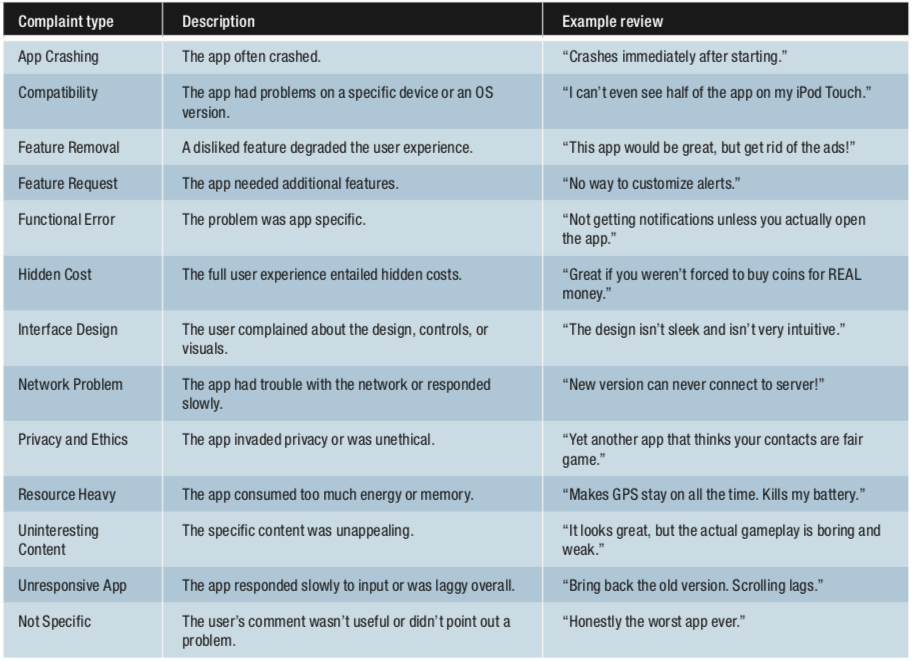
\includegraphics[width=\textwidth]{images/mobile_users_complaints_table}
    \caption[Reclamações mais comuns de usuários de aplicações móveis]
    {Reclamações mais comuns de usuários de aplicações móveis \cite{Khalid2015}}
    \label{fig:mobile_users_complaints_table}
\end{figure}

Infere-se da tabela acima que um usuário de aplicações móveis espera que a 
aplicação

\begin{itemize}
\setlength\itemsep{0em}
\item Não trave;
\item Seja compatível com seu dispositivo;
\item Atenda somente às funcionalidades esperadas;
\item Explicite as cobranças utilizadas na aplicação; 
\item Possua uma boa interface gráfica;
\item Possua boa conectividade com a Internet;
\item Atenda às condições de privacidade e ética esperadas da aplicação;
\item Consuma o mínimo possível de recursos de hardware;
\item Seja interessante;
\item Seja responsiva.
\end{itemize}
 
 \section{Web Service}
 Um item notório na publicação do IEEE \cite{Khalid2015} previamente citada
  é a conectividade com a Internet. Apesar de a pesquisa ter sido feita nos Estados 
  Unidos, a realidade no Brasil não é muito diferente. Segundo o IBGE \cite{ibge2015}, 
 em 2014, pela primeira vez, o uso do telefone celular para acessar a Internet 
 ultrapassou o uso de microcomputador nos domicílios brasileiros. \cite{ibge2015}
 Em 2015, esse cenário se repetiu no País. \cite{ibge2015} Conforme o mostra
 gráfico a seguir:
 
 \begin{figure}[htb]
    \centering
    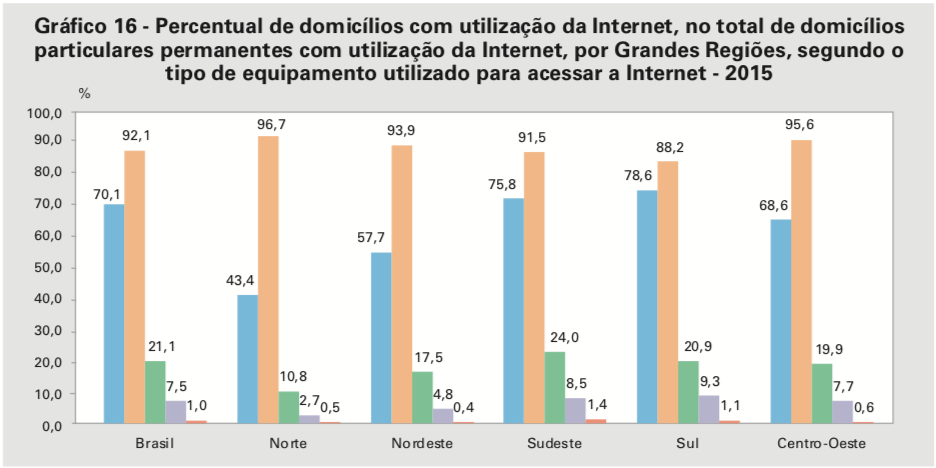
\includegraphics[width=\textwidth]{images/ibge_celulares_computadores}
    \caption[Utilização de internet via dispositivos móveis versus computadores]
    {Utilização de internet via dispositivos móveis versus computadores \cite{ibge2015}}
    \label{fig:ibge_celulares_computadores}
\end{figure}

Ao comunicar-se com a Internet um aplicativo passa a fazer parte de um web 
service.

Um web service é um sistema de software designado a suportar interações
máquina-com-máquina sobre uma rede de computadores. \cite{Ferris2004}
Num sistema web existem dois agentes: uma máquina que provém um serviço,
conhecida como servidor, e uma máquina que requisita o serviço, chamada 
de cliente. Existem diversas arquiteturas de comunicação entre o cliente e o 
servidor, uma delas é através de APIs. \cite{Tanenbaum2011}

\begin{figure}[H]
    \centering
    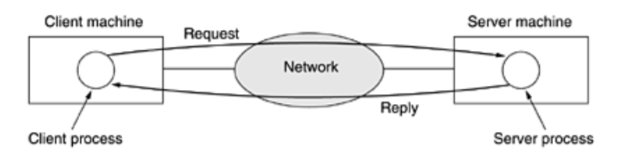
\includegraphics[scale=0.8]{images/client_server}
    \caption[Arquitetura Cliente/Servidor]
    {Arquitetura Cliente/Servidor \cite{Tanenbaum2011}}
    \label{fig:client_server}
\end{figure}


\subsection{Rede de computadores}
Para viabilizar a comunicação entre o cliente e o servidor, 
um web service necessita de uma rede de computadores.
Uma rede de computadores é um conjunto de computadores autônomos 
interconectados por uma única tecnologia. \cite{Tanenbaum2011}
A World Wide Web (Web), por exemplo, é uma rede de redes de 
computadores, \cite{Tanenbaum2011} já que utiliza mais de uma tecnologia em suas 
conexões.
A maioria das redes é organizada como uma pilha de camadas ou níveis, 
colocadas umas sobre as outras. \cite{Tanenbaum2011} 
O objetivo de cada camada é oferecer determinados serviços às camadas superiores, 
isolando essas camadas dos detalhes de implementação desses recursos. 
\cite{Tanenbaum2011}

A camada n de uma máquina se comunica com a camada n de outra máquina. 
Coletivamente, as regras e convenções usadas nesse diálogo são conhecidas como 
o protocolo da camada n. \cite{Tanenbaum2011}
\begin{figure}[H]
    \centering
    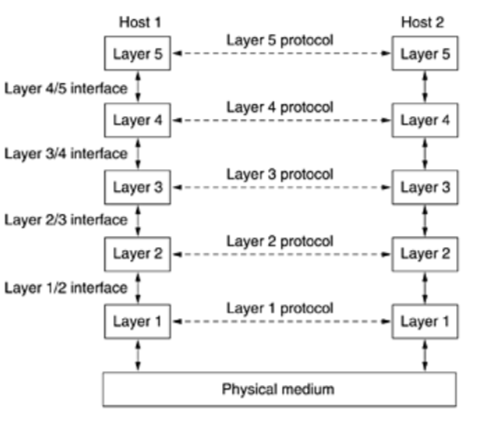
\includegraphics[scale=1.2]{images/layers_protocols}
    \caption[Camadas e protocolos de uma rede de computadores]
    {Camadas e protocolos de uma rede de computadores \cite{Tanenbaum2011}}
    \label{fig:layers_protocols}
\end{figure}

Um protocolo amplamente conhecido é o HTTP que é
usado na Camada de Aplicação do modelo de referência TCP/IP
e cuja principal função é buscar páginas na World Wide Web. \cite{Tanenbaum2011}

\subsection{API}
Pessoas usam aplicações via Interfaces Gráficas. Já aplicações usam outras 
aplicações via API (do inglês, Application Programming Interface). \cite{Biehl2015}
APIs provêm as capacidades essenciais para conectar, extender e integrar 
software. \cite{Biehl2015}
Com uma mesma API é possível acessar os serviços de um servidor em muitos clientes 
distintos.

\begin{figure}[H]
    \centering
    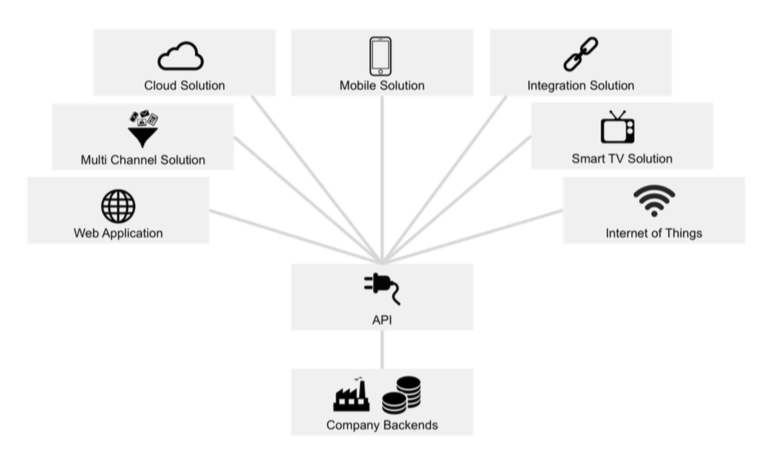
\includegraphics[scale=1]{images/api_architecture}
    \caption[Arquitetura de uma API]
    {Arquitetura de uma API \cite{Biehl2015}}
    \label{fig:api_architecture}
\end{figure}

Existem diversas estilos de arquiteturas de implementação de APIs. Dentre eles,
o REST (do inglês Representation State Transfer), o RPC (do inglês, Remote 
Procedure Call) e o SOAP (do inglês, Simple Object Access Protocol).
Sendo hoje em dia as mais comuns o REST e o SOAP. \cite{Castillo2011}

\subsubsection{REST}
REST é um estilo de arquitetura para serviços que define um conjunto de restrições
e acordos na arquitetura. Um serviço que cumpre as resgras REST é chamado de
RESTful. \cite{Biehl2015}
O REST foi desenvolvido para fazer uso otimizado de infraestruturas baseadas 
em HTTP.  \cite{Biehl2015}

Mensagens REST possuem pouco payload, o que é adequado para aplicações 
móveis. \cite{Wagh2012}

\subsubsection{SOAP}
SOAP é o protocolo padrão de interface para web services proposto pelo W3C e
é aplicável a qualquer protocolo da camada de aplicação (HTTP, SHTTP, FTP, 
etc). \cite{Castillo2011}

Entretanto, as mensagens SOAP contém muitos meta dados e apenas suportam
estruturas verbosas de XML para solicitações e respostas. Além disso, devido
ao seu grande tamanho, serviços SOAP são considerados complexos
para ambos os provedores e consumidores de serviços. \cite{Biehl2015}

\newpage 
\section{Criação de projetos para Android e para iOS}
\subsection{Android Studio}
O Android Studio é a IDE oficial para desenvolvimento de aplicativos para 
Android.

Depois de fazer o download e de instalar o software, o primeiro passo 
para criar uma aplicação Android é escolher a opção: 
\enquote{Start a new Android Studio project} ou equivalente caso o idioma de instalação 
não seja o inglês.

\begin{figure}[H]
    \centering
    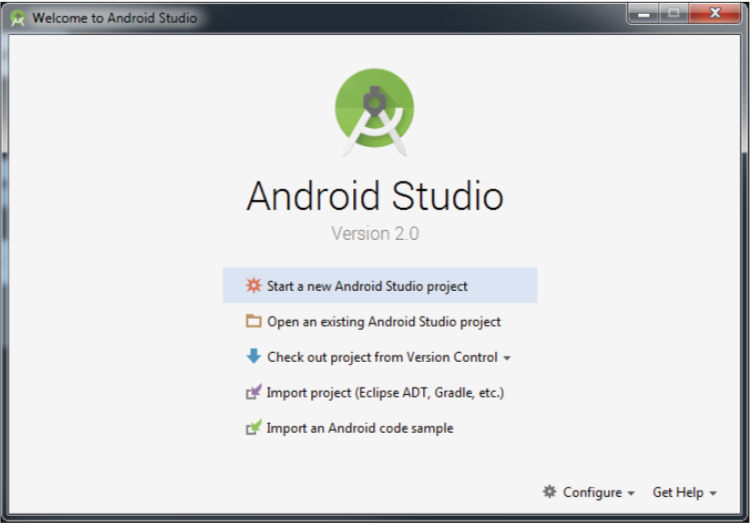
\includegraphics[scale=0.8]{images/android_studio_1}
    \caption[Novo projeto no Android Studio - Passo 1]
    {Novo projeto no Android Studio - Passo 1 \cite{DiMarzio2016}}
    \label{fig:android_studio_1}
\end{figure}

Em seguida, deve-se nomear a aplicação, bem como escolher o domínio,
o diretório onde os arquivos ficarão e o nome do pacote.

\begin{figure}[H]
    \centering
    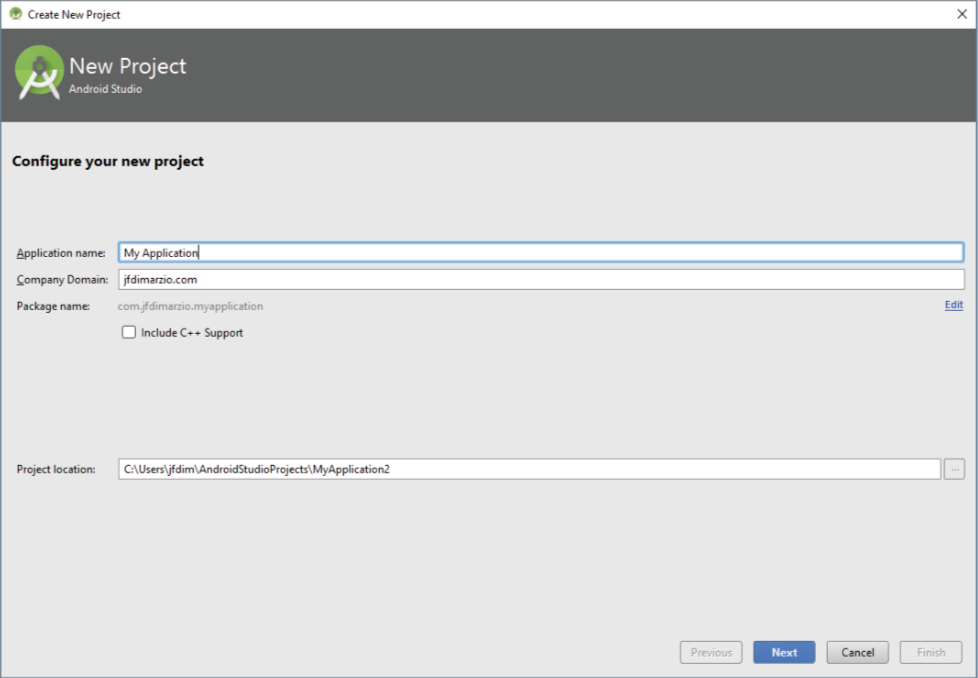
\includegraphics[scale=0.65]{images/android_studio_2}
    \caption[Novo projeto no Android Studio - Passo 2]
    {Novo projeto no Android Studio - Passo 2 \cite{DiMarzio2016}}
    \label{fig:android_studio_2}
\end{figure}

Após, escolhe-se o SDK mínimo para cada opção que a aplicação será 
utilizada dentre: smartphones e tablets, wear e etc. O escopo deste trabalho se
limita a smartphones e tablets. Quanto menor for a versão do SDK escolhido,
maior será o número de dispositivos que suportarão a aplicação.

\begin{figure}[H]
    \centering
    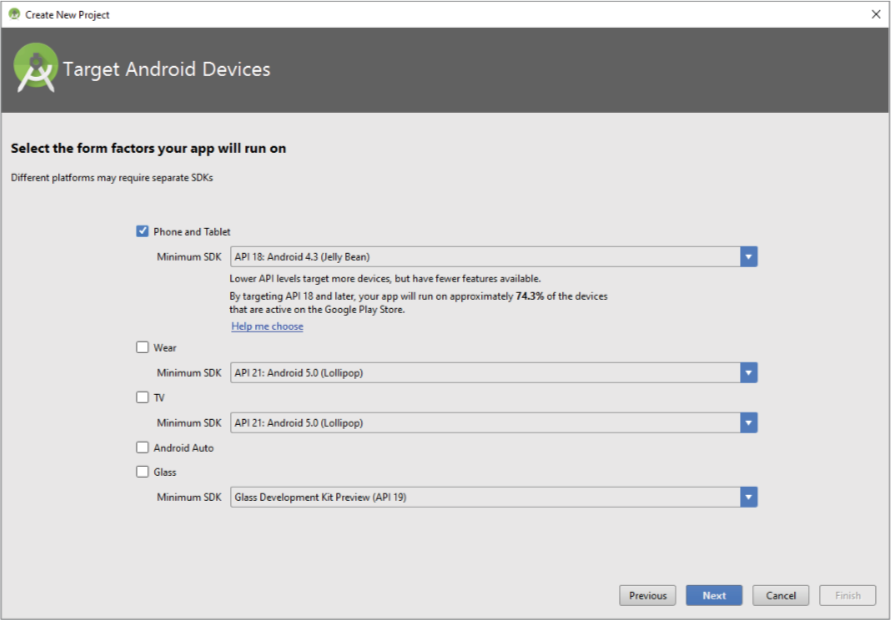
\includegraphics[scale=0.65]{images/android_studio_3}
    \caption[Novo projeto no Android Studio - Passo 3]
    {Novo projeto no Android Studio - Passo 3 \cite{DiMarzio2016}}
    \label{fig:android_studio_3}
\end{figure}

Feito isso, aparecerão algumas opções de Activity para serem adicionadas à 
aplicação. O modelo mais básico é o \enquote{Empty Activity} e este modelo deve
ser o escolhido num primeiro momento até que se obtenha um maior conhecimento
da plataforma.

\begin{figure}[H]
    \centering
    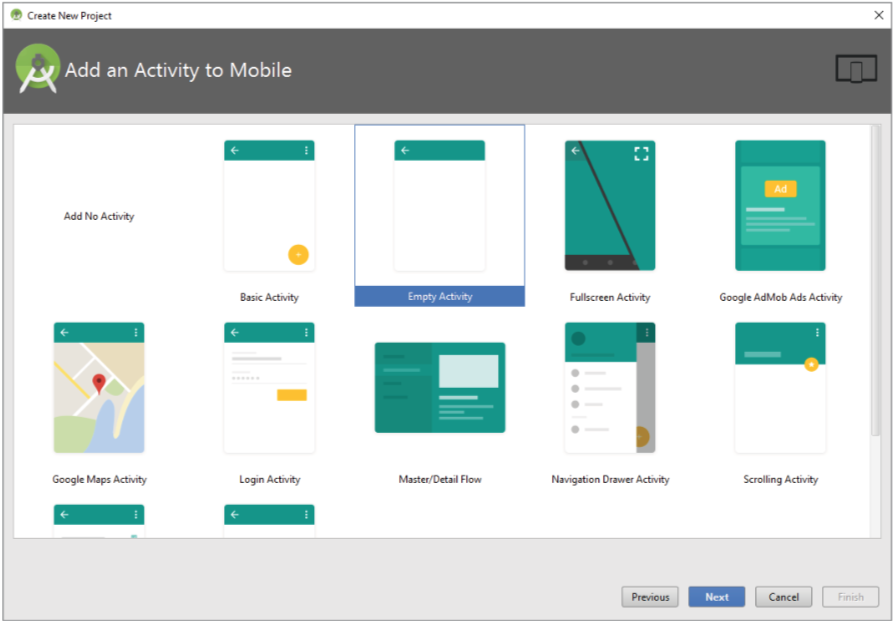
\includegraphics[scale=0.65]{images/android_studio_4}
    \caption[Novo projeto no Android Studio - Passo 4]
    {Novo projeto no Android Studio - Passo 4 \cite{DiMarzio2016}}
    \label{fig:android_studio_4}
\end{figure}

A IDE será iniciada e alguns arquivos serão criados e podem ser selecionados
no navegador à esquerda. Os detalhes de cada um 
desses arquivos será explicado com mais detalhes no próximo capítulo.

\begin{figure}[H]
    \centering
    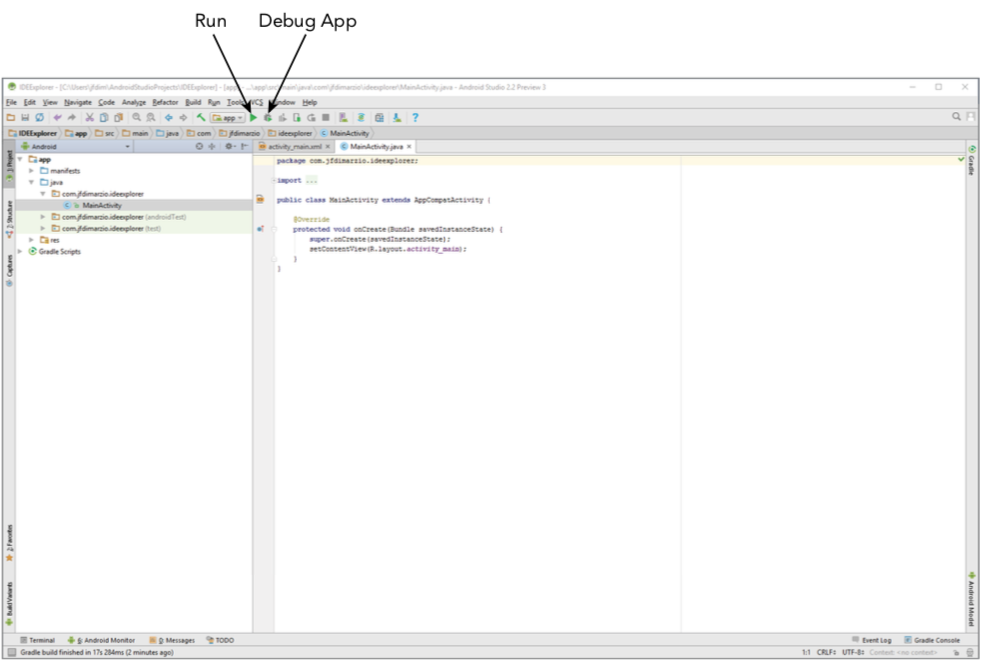
\includegraphics[width=\textwidth]{images/android_studio_5}
    \caption[IDE Android Studio]
    {IDE Android Studio \cite{DiMarzio2016}}
    \label{fig:android_studio_5}
\end{figure}

O código pré-escrito cria uma Activity vazia. Para visulizá-la basta clicar no 
botão \enquote{Run App}. É possível rodar as aplicações tanto em dispositivos 
físicos, quanto em dispositivos vituais.

\begin{figure}[H]
    \centering
    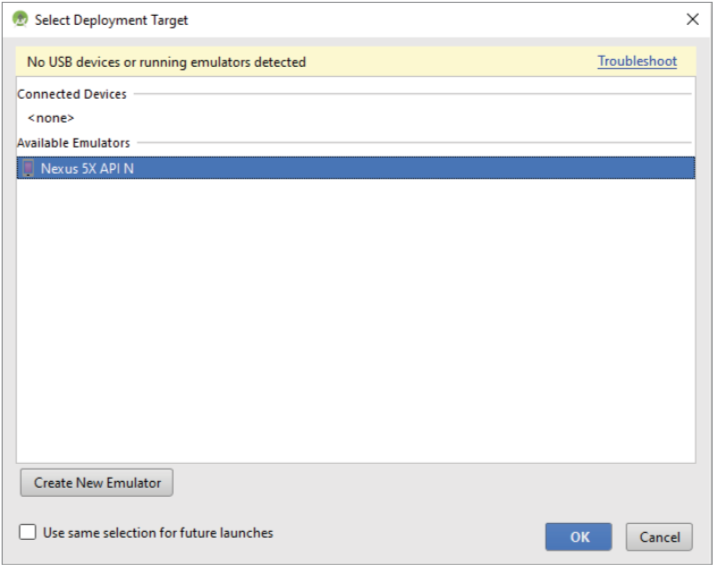
\includegraphics[scale=0.8]{images/android_studio_avd}
    \caption[Selecionar dispositivo no Android Studio]
    {Selecionar dispositivo no Android Studio \cite{DiMarzio2016}}
    \label{fig:android_studio_avd}
\end{figure}

Compilando o exemplo criado em \cite{DiMarzio2016} num dispositivo virtual,
 obtevê-se o seguinte resultado:

\begin{figure}[H]
    \centering
    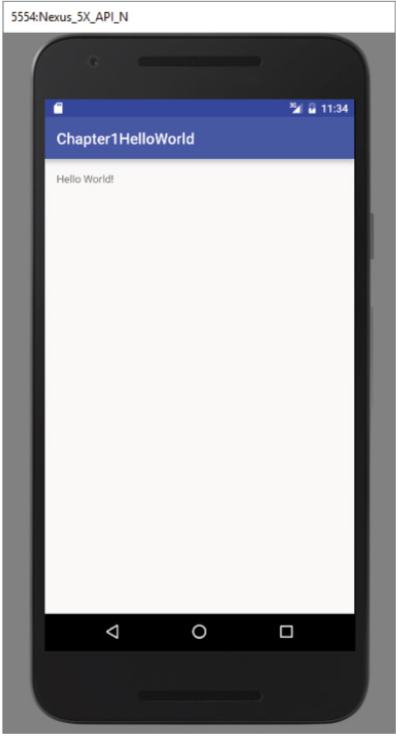
\includegraphics[scale=0.8]{images/android_studio_primeiro_programa}
    \caption[Exemplo com Empty Activity]
    {Exemplo com Empty Activity \cite{DiMarzio2016}}
    \label{fig:android_studio_primeiro_programa}
\end{figure}

\subsection{XCode}
